%!TEX root = Thesis.tex

\chapter{Parallel circuit performance exploration for circuit sizing via genetic algorithm}\label{chap:PAGE}
  \section{Introduction}\label{sec:PAGEIntro}
    To simplify the analog sizing problem, in this chapter, we treat the analog circuit performance exploration problem as a searching process. According to the complexity for searching multi-objective problem, a framework which integrates global and local search is considered. Moreover, we also investigate that evolutionary algorithm such as genetic algorithm is workable for exploration in high-dimensional performance space. Background knowledges for hierarchical framework and genetic algorithm are as follows.
    \subsection{Problem Description} 
      State-of-the-art acknowledges a collection of Pareto-fronts which sketch the performance space, later an optimal point is selected for local search problem, which did not mention that how to define optimal point among the space. Instead of collecting the performance space information, this paper aggressively define performance limit as exploration main objective:

      \newtheorem{defi}{Definition}
      
      \begin{defi}
        {\bf Circuit Performance}: A circuit performance is consisted of multiple values, such as DC voltage gain, 3dB gain bandwidth and power consumption. Different circuit has different circuit performance target.
      \end{defi}

      \begin{defi}
        {\bf Performance limit exploration for global search problem}: Given a circuit design equation in posynomial forms with a set of feasible circuit-level design variables and a set of circuit performance constraints, perform convex optimization with different performance value to traverse the utmost performance space of the given circuit.\footnote{Here, the maximum and minimum performance values are investigated whether feasible or not. Therefore, it can tell that the global search process generates a space of feasible performances and each represents a set of optimal design variables. Although the global search obtains a space of performance, it is not the exact optimal solution. The global search is a preparation for later local search. This work proposes a flexible non-uniform stochastic simulation as local search for optimal sizing solution. }
      \end{defi}


      \begin{defi}
        {\bf Stochastic simulation for local search:} A set of feasible performance is re-targeted to corresponding design variables. The local search practices a stochastic SPICE simulation w.r.t. these selected design variables. 
      \end{defi}
    \subsection{Hierarchical Circuit Performance Exploration Methodology\cite{PerfMap_ISQED2011}}
      To cope with complicated analog sizing problem, a process to find solutions for multiple performance targets can be divided into bi-direction search stages. Generally, in the design flow of analog IC, which begins from performance level, through circuit (netlist) level and then implements in device level. In performance level, designers specify the circuit behavior as performance, such as voltage gain, frequency bandwidth and output power. later, the circuit level parameters and describe the netlist topology. Meanwhile, the device level shows the device information which connects to physical layout. 

      The bottom-up global search stage begins from device model level to feasible performance space. A range of feasible performance are transfer back to design variables via local search, and then performing a guided stochastic simulation for optimality. In detail, the hierarchical search process are 1) Device Fitting, 2) Performance Space Exploration, 3) Geometric Design Re-targeting and 4) Stochastic Fine Tuning. The enhancement of such hierarchical search methodology is delivered in Section~\ref{sec:GPEF}
    \subsection{Parallel Genetic Algorithm}
      \begin{figure}[t]
        \centering
        \centerline{
          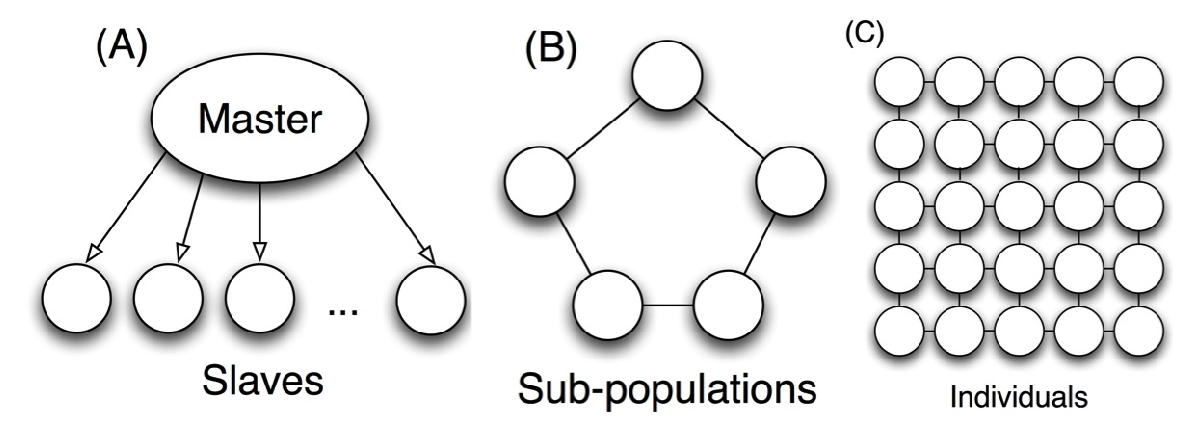
\includegraphics[width=0.7\textwidth]{Fig/Chapter2/PGA_reduced.eps}
        }
        \caption{Three different models of parallel genetic-algorithm: (A) master-slave, (B) coarse-grained, and (C) fine-grained.}
        \label{fig:PGA}
        \end{figure}

      Different from traditional genetic algorithm, the basic idea of parallel genetic algorithm is divide-and-conquer flavor, which can be applied to genetic algorithm in many different variations. Alba et al.~\cite{SurveyDistPGA1997} and Cant-Paz \cite{SurveyPGA1997} classify the parallel genetic algorithm into three main types: (1) master-slave genetic algorithm, (2) fine-grained genetic algorithm, and (3) coarse-grained genetic algorithm. Fig.~\ref{fig:PGA} shows three types parallel genetic-algorithm as mentioned above.
          
      Parallel genetic algorithm is not just parallel versions of traditional genetic algorithm, parallel genetic algorithm can actually reach the ideal goal via various parameters setting. Multi-objective optimization problem can achieved via different parameter and exchange their individuals between each sub-population.

  \section{Genetic Performance Exploration Flow}\label{sec:GPEF}
  \section{Probablistic Simulation}\label{sec:ProbSimu}
  \section{Experimental Results}\label{sec:PAGEExp}

  
  \section{Summary}\label{sec:PAGESum}